\documentclass[tikz, footheight=2em]{beamer}
\usetheme[hideothersubsections]{Hannover}
\usepackage[T1]{fontenc}
\usepackage[utf8]{inputenc}
\usepackage{amssymb}
\usepackage{amsthm}
\usepackage{amsmath}
\usepackage{stmaryrd}
\usepackage{color,graphicx}
\usepackage{gensymb}
\usepackage{tikz,pgfplots}
\usepackage{algorithm}
\usepackage{algpseudocode}
\usepackage{float}
\usepackage{subfig}
\usepackage{tabulary}
\usepackage{graphicx}

\DeclareMathOperator{\card}{card}
\DeclareMathOperator{\argmax}{argmax}
\DeclareMathOperator{\uniform}{Uniform}

\usecolortheme{dolphin}

\title{Tetris par Q learning}
\author{C.~Cousin, G.~Hondet, L.~Pineau, B.~Viry}
\date{}

\usetikzlibrary{patterns,arrows,positioning}
\tikzset{
    %Define standard arrow tip
    >=stealth',
    %Define style for boxes
    punkt/.style={
           rectangle,
           rounded corners,
           draw=black, very thick,
           text width=6.5em,
           minimum height=2em,
           text centered},
    % Define arrow style
    pildwn/.style={
           <-,
           thick,
           shorten <=2pt,
           shorten >=2pt,},
    pilup/.style={
           ->,
           thick,
           shorten <=2pt,
           shorten >=2pt,}
}

% ----------------------------------------------------------
% nuremotation des pages -----------------------------------
% ----------------------------------------------------------
\def\swidth{1.6cm}
\setbeamersize{sidebar width left=\swidth}
\setbeamertemplate{sidebar left}
{%
  {\usebeamerfont{title in sidebar}
    \vskip1.5em
    \usebeamercolor[fg]{title in sidebar}
    \insertshorttitle[width=\swidth,center,respectlinebreaks]\par
    \vskip1.25em
  }
  {
    \usebeamercolor[fg]{author in sidebar}
    \usebeamerfont{author in sidebar}
    \insertshortauthor[width=\swidth,center,respectlinebreaks]\par
    \vskip1.25em
  }
  \hbox to2cm{\hss\insertlogo\hss}
  \vskip1.25em
  \insertverticalnavigation{\swidth}
  \vfill
  \hbox to2cm{\hskip0.6cm\usebeamerfont{subsection in
      sidebar}\strut\usebeamercolor[fg]{subsection in
      sidebar}\insertframenumber /\inserttotalframenumber\hfill}
  \vskip3pt
}
% ----------------------------------------------------------


\begin{document}

\frame{\titlepage}

\AtBeginSection[]
{%
  \begin{frame}
    \frametitle{Plan}
    \tableofcontents[currentsection]
  \end{frame}
}

\section*{Introduction}
\begin{frame}[c]{Introduction}
  \begin{center}
    \begin{minipage}[c]{0.4\linewidth}
      \includegraphics[height=6cm]{tetris.png}
    \end{minipage}
    \begin{minipage}[c]{0.4\linewidth}
      \includegraphics[height=3cm]{alphago.jpg}
    \end{minipage}
  \end{center}
\end{frame}

\section{Apprentissage}
\subsection{Apprentissage par renforcement}
\begin{frame}{Apprentissage par renforcement}
  \begin{block}{Principe}
    Un agent évoluant dans son environnement se voit attribuer des
    récompenses en fonction de la pertinence de ses actions.
    \begin{figure}[h]
      \begin{center}
        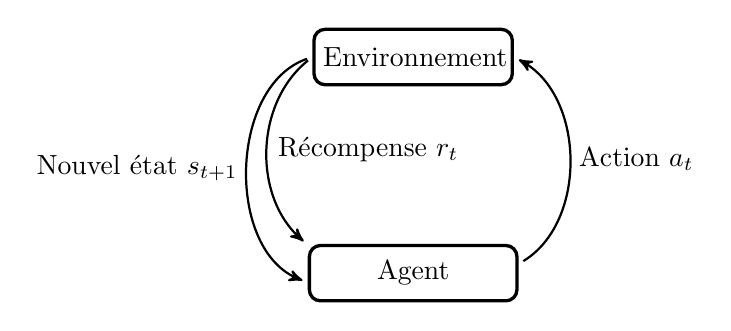
\begin{tikzpicture}[node distance=1cm, auto,]
         %nodes
          \node[punkt] (env) {Environnement};
          \node[punkt, inner sep=5pt,below=2cm of env]
          (agent) {Agent}
          edge[pilup,bend right=60] node[right] {Action \(a_t\)} (env.east)
          edge[pildwn,bend left=70] node[left] {Nouvel état \(s_{t+1}\)}
          (env.west)
          edge[pildwn,bend left=50] node[right] {Récompense \(r_t\)} (env.west);
        \end{tikzpicture}
      \end{center}
      \caption{Principe d'apprentissage par renforcement, à l'instant \(t\)}
      \label{fig:reinforcement_learning}
    \end{figure}
  \end{block}
\end{frame}


\subsection{Q learning}

\begin{frame}{Q learning}
  \begin{block}{Agent}
    Utilise une matrice Q pour stocker les espérances de récompense à long
    terme (somme des récompenses d'une partie).
  \end{block}
  \begin{itemize}
    \item Les colonnes de la matrice correspondent aux actions.
    \item Les lignes de la matrice correspondent aux états.
  \end{itemize}
\end{frame}

\subsection{Choix de l'action}

\begin{frame}{État}
  Données utiles de l'environnement pour jouer une action.

  \begin{exampleblock}{Dans notre cas}
    Les deux plus hautes lignes non vides du plateau.
  \end{exampleblock}
  \begin{block}{Obtention}
    \[
      \text{état} = \text{plateau} + \text{pièce} =
      \pause{} \in \mathbb{N}
    \]
  \end{block}
\end{frame}

\begin{frame}{Choix de l'action}
    \(Q(s, a)\) approxime la récompense à long terme,
    \pause{}
    \[ \text{action choisie} = \underset{a}{\argmax} Q(s, a) \]
    \pause{}
  \begin{algorithm}[H]
      \caption{Choix de l'action}\label{alg:action}
      \begin{algorithmic}
        [1]
        \Procedure{ChooseAction}{$Q$, $s$, $\mathcal{A}$}
        \State{} tirage \(\gets \uniform([0, 1])\)
        \If{tirage \(> \epsilon\)}
        \Return{\(\argmax_{a\in\mathcal{A}} Q(s, a)\)}
        \Else{}
        \Return{\(\uniform(\mathcal{A})\)}
        \EndIf{}
        \EndProcedure{}
      \end{algorithmic}
  \end{algorithm}
\end{frame}

\begin{frame}[c]{Exploitation v exploration}
  \begin{description}[Exploitation]
    \item[Exploration] balayer toutes les actions possibles
    \item[Exploitation] tirer profit de l'apprentissage
  \end{description}
  \pause{}
  \[ \Downarrow \]
  \[ \text{Choix de } \epsilon \]
  \pause{}
  \begin{block}{Compromis}
    Peut-être assuré par une variation d'\(\epsilon\) au cours des parties.
  \end{block}
\end{frame}

\section{Environnement Tetris}
\subsection{Tetromino}
\begin{frame}[c]{Tetromino}
  \begin{block}{Représentation}
    Matrice \(2 \times 2\) d'entiers
  \end{block}
  \begin{figure}[h]
    \centering
    \subfloat[Diagonale] {%
      
\begin{tikzpicture}
        \fill[color=magenta] (0,0) rectangle (1,1);
        \fill[color=magenta] (0,0) rectangle (-1,-1);
        \draw (-1,1) rectangle (1,-1);
      \end{tikzpicture}
    }\qquad
    \subfloat[L] {%
      
\begin{tikzpicture}
        \fill[color=cyan] (0,0) rectangle (1,1);
        \fill[color=cyan] (0,0) rectangle (-1,-1);
        \fill[color=cyan] (0,0) rectangle (-1,1);
        \draw (-1,1) rectangle (1,-1);
      \end{tikzpicture}
    }\qquad
    \subfloat[Carré] {%
      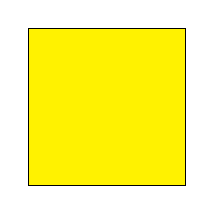
\begin{tikzpicture}
        \fill[color=yellow] (0,0) rectangle (1,1);
        \fill[color=yellow] (0,0) rectangle (-1,-1);
        \fill[color=yellow] (0,0) rectangle (-1,1);
        \fill[color=yellow] (0,0) rectangle (1,-1);
        \draw (-1,1) rectangle (1,-1);
      \end{tikzpicture}
    }\\
    \subfloat[Barre] {%
      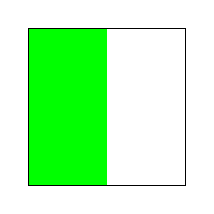
\begin{tikzpicture}
        \fill[color=green] (0,0) rectangle (-1,-1);
        \fill[color=green] (0,0) rectangle (-1,1);
        \draw (-1,1) rectangle (1,-1);
      \end{tikzpicture}
    }\qquad
    \subfloat[Point] {%
      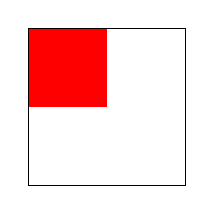
\begin{tikzpicture}
        \fill[color=red] (0,0) rectangle (-1,1);
        \draw (-1,1) rectangle (1,-1);
      \end{tikzpicture}
    }
    \caption{Liste des tetrominos}\label{fig:tetrolist}
  \end{figure}
\end{frame}

\subsection{Mouvement}
\begin{frame}[c]{Mouvement}
  \begin{block}{Définition}
    Données utiles au placement d'un tetromino sur le plateau.
    \pause{}
    \[ \text{mouvement} = \text{orientation} + \text{translation} \]
  \end{block}
  \pause{}
  \begin{block}{Types}
    \begin{itemize}
      \item translation \(\in \llbracket 0, 4 \rrbracket\)
      \item orientation \(\in \{\)North, South, East, West\(\}\)
    \end{itemize}
  \end{block}
\end{frame}

\subsection{Gestion du plateau}
\begin{frame}[c]{Réalisation du mouvement et conséquences}
  \begin{block}{Plateau}
    Matrice d'entiers de largeur 6.
  \end{block}
  \begin{block}{Placement vertical}
    Évaluation des collisions : collision \(\rightarrow\) placé en amont
  \end{block}
\end{frame}
\begin{frame}[c]{Ligne pleine}
  \begin{block}{Lignes pleines}
    Ligne remplie enlevée du jeu
  \end{block}
  \begin{alertblock}{Tetromino flottant}
    schema here. Pour résoudre : un ensemble d'orientations par tetromino.
  \end{alertblock}
\end{frame}

\section{Évolution de l'agent}
\subsection{Récompense}
\begin{frame}[c]{Récompense ou pénalité}
  \begin{block}{Motivation}
    Quantifie la pertinence du mouvement effectué.
  \end{block}
  \pause{}
  \begin{block}{Objectif de l'agent}
    Minimiser la hauteur finale.
  \end{block}
  \pause{}
  \[ R(\delta h) = k \cdot \delta h, k < 0 \]
  avec \(\delta h =\) hauteur après coup \(-\) hauteur avant coup.
\end{frame}
\subsection{Mise à jour}
\begin{frame}[c]{Mise à jour}
  \begin{block}{Besoin}
    Prendre en compte les récompenses pour modifier le comportement de l'agent.
  \end{block}
  \pause{}
  \[
    Q(s_t, a_t) \leftarrow Q(s_t,a_t) + \alpha
    [r_t + \gamma \max_{a_{t+1}} Q(s_{t+1},a_{t+1}) - Q(s_t,a_t)]
  \]
\end{frame}

\subsection{Paramétrage}
\begin{frame}[c]{Paramètres}
  \begin{block}{Taux d'apprentissage \(\alpha\)}
    Doit vérifier \(\sum_{k} \alpha_k = \infty, \quad
    \sum_k \alpha_k^2 < \infty \).
    \pause{}
    Ici, \[ \alpha_k = \frac{1}{1 + Ck} \]
    Nous agirons sur \(C\).
  \end{block}
  \pause{}
  \begin{block}{Vision de l'agent \(\gamma\)}
    Prise en compte des récompenses futures, \(\in [0,1]\).
    \pause{}
    \begin{itemize}
      \item \(\gamma \to 0 \implies\) Agent myope, pas de considération des
        récompenses futures.
      \item \(\gamma \to 1 \implies\) Valorise autant les récompenses futures
        que la récompense immédiate.
    \end{itemize}
  \end{block}
\end{frame}

\begin{frame}[c]{Qualification de l'agent}
  \begin{description}[Hauteur finale]
    \item[Décroissance] temps de passage au-dessous d'un seuil
    \item[Hauteur finale] hauteur une fois celle-ci stabilisée
    \item[Stabilité] variation des hauteurs finales autour de la moyenne 
  \end{description}
  \begin{figure}[H]
    \begin{tikzpicture}
      \begin{axis}[
          line width=0.05, mark size = 0.1,
          height = 0.5\linewidth,
          width = \linewidth,
          xlabel = jeux, ylabel = hauteur fin de jeu
        ]
        \addplot+ table [
          x expr = {\lineno}, y index = 0,
        ]
        {data/gamma.dat};
      \end{axis}
    \end{tikzpicture}
  \end{figure}
\end{frame}

\begin{frame}[c]{Qualification de l'agent}
  \begin{description}[Hauteur finale]
    \item[Décroissance] temps de passage au-dessous d'un seuil
    \item[Hauteur finale] hauteur une fois celle-ci stabilisée
    \item[Stabilité] variation des hauteurs finales autour de la moyenne 
  \end{description}
  \begin{figure}[H]
    \begin{tikzpicture}
      \begin{axis}[
          line width=0.05, mark size = 0.1,
          height = 0.5\linewidth,
          width = \linewidth,
          xlabel = jeux, ylabel = hauteur fin de jeu
        ]
        \addplot+ table [
          x expr = {\lineno}, y index = 0,
        ]
        {data/gamma.dat};
        \addplot[domain=0:512]{100};
      \end{axis}
    \end{tikzpicture}
  \end{figure}
\end{frame}

\begin{frame}[c]{Résultats}
  \begin{figure}[H]
    \begin{tikzpicture}
      \begin{axis}[line width=0.05, mark size = 0.1,
          legend entries={.002,.068,.134,.2},
          xlabel = {jeux},
          ylabel = {hauteur fin de jeu},
          title = Apprentissages avec différents \(\epsilon\),
        ]
        \foreach \i in {0,1,...,3}{%
          \addplot+ table [x expr = {\lineno}, y index = \i]
          {data/epsilon_wide.dat};
        }
      \end{axis}
    \end{tikzpicture}
  \end{figure}
\end{frame}

\begin{frame}[c]{Tests paramètres}
  \begin{block}{Protocole}
    \begin{itemize}
      \item Seuil défini par nombre de jeux pour passer en dessous d'une
        hauteur finale fixée.
      \item Moyenne (moy.) et écarts types (e.t.) calculés sur les dernières
        parties.
    \end{itemize}
  \end{block}
  \pause{}
  \begin{table}
    \centering
    \begin{tabulary}{\linewidth}{|C|r|r|r||r|r|r|}
      \hline
      & \(C\) & \(\epsilon\) & \(\gamma\) & Moy. & E.t.\ & Seuil\\
      \hline
      Moy. & 0.001 & 0.0025 & 0.65 & 1.14 & 1.08 & 68\\
      \hline
      E.t.\ & 0.001 & 0.0025 & 0.65 & 1.14 & 1.08 & 68\\
      \hline
      Seuil & 0.0007 & 0.0005 & 1 & 3.14 & 2.96 & 29\\
      \hline
    \end{tabulary}
    \caption{Valeurs optimales}\label{tab:param}
  \end{table}
\end{frame}


\section{Valuation}
\begin{frame}[c]{Fonction de valuation}
  \begin{block}{Motivation}
    S'affranchir des contraintes mémoires liées à la Q matrice. Le nouvel état
    contient le plateau entier.
  \end{block}
  \pause{}
  \begin{block}{Agent}
    Application linéaire \(V\) donnant l'espérance de récompense.
  \end{block}
  \pause{}
  \begin{exampleblock}{Features}
    Caractéristiques utiles du plateau pour estimer l'espérance de récompense.
    E.g.\ Nombre de trous, hauteur de la dernière pièce tombée.
  \end{exampleblock}
  \pause{}
  \begin{block}{Apprentissage}
    Modification des poids composant \(V\) par descente de gradient.
  \end{block}
\end{frame}

\section*{Conclusion}
\begin{frame}[c]{Conclusion}
  Résultats concluant concernant le Q learning.
\end{frame}
\end{document}
